\documentclass[11pt]{article}

\usepackage[margin=1in]{geometry}
\usepackage{amsmath,amssymb,amsthm}
\usepackage{graphicx}
\usepackage{hyperref}
\hypersetup{hidelinks}

\newtheorem{theorem}{Theorem}
\newtheorem{lemma}[theorem]{Lemma}
\newcommand{\CB}{\operatorname{CB}}
\newcommand{\cc}{\operatorname{cc}}
\newcommand{\dH}{d_{\mathrm H}}

\title{Compact affine actions reduce to the linear-isometric case\\
for hyperspaces of bounded convex sets}
\author{Run \texttt{fa\_banach\_001}, lane 6}
\date{August 12, 2026}

\begin{document}
\maketitle

\begin{abstract}
Jonard-P\'erez asks whether $\CB(L)$ is a $G$-equivariant absolute extensor
when a compact group $G$ acts continuously and affinely on a Banach space
$L$ and the induced action on $\CB(L)$ is continuous.  We give an
affirmative answer.  Haar-averaging any orbit produces a fixed point $c$.
Translation by $c$ conjugates the affine action to a continuous linear
action, and the equivalent norm
\[
  \|x\|_G=\sup_{g\in G}\|gx\|
\]
makes that action isometric.  Equivalent norms induce bi-Lipschitz
equivalent Hausdorff metrics on $\CB(L)$, so the assumed hyperspace
continuity is preserved.  The problem is therefore exactly the
linear-isometric case settled by Theorem~5.1 of the source paper.
\end{abstract}

\section{Source question and available theorem}

For a Banach space $L$, let $\CB(L)$ be the hyperspace of all nonempty closed,
bounded, convex subsets of $L$, equipped with the Hausdorff metric.  The
source is N. Jonard-P\'erez, \emph{Equivariant absolute extensor property on
hyperspaces of convex sets}, arXiv:1401.2653v2 \cite{Source}.  Its final
Question~6.2 is reproduced below.

\begin{center}

\includegraphics[width=0.98\textwidth]{figures/open_question_crop.png}
\end{center}

The source had already proved the following linear-isometric result.  In its
terminology, a Banach $G$-space is a Banach space on which $G$ acts linearly
and the norm is $G$-invariant.

\begin{center}
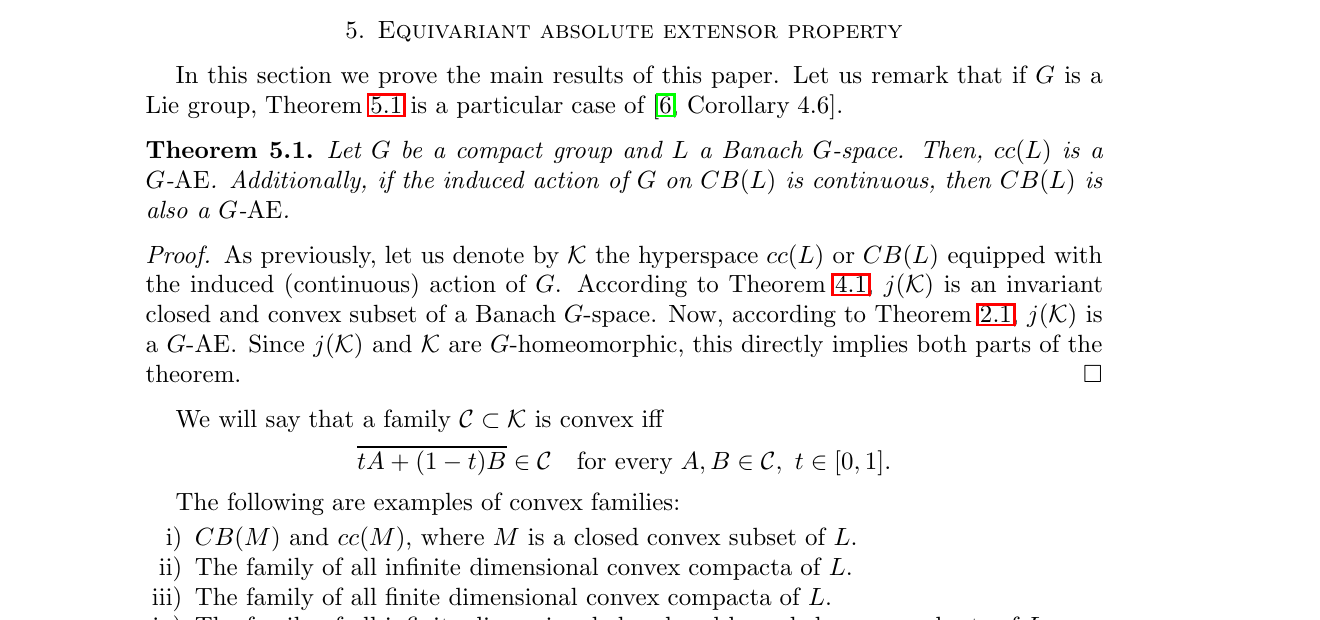
\includegraphics[width=0.98\textwidth]{figures/source_theorem_5_1_crop.png}
\end{center}

Thus the only issue is whether the compact affine action in Question~6.2 can
be placed in that setting without changing the topology of $\CB(L)$.  It can.

\section{Proof intuition}

The source tries to replace the affine action by the orbit-map embedding
$x\mapsto(g\mapsto gx)$ into $C(G,L)$.  That map need not be uniformly
continuous, which matters for Hausdorff hyperspaces of arbitrary bounded
sets.  A compact affine action admits a more direct reduction.  Average one
orbit against Haar probability measure.  Its barycenter is fixed by the
whole group.  Once that point is declared to be the origin, the action is
linear.  Compactness then supplies a uniformly equivalent invariant norm.
Unlike the orbit-map embedding, translation and equivalent renorming are
bi-Lipschitz on the entire hyperspace of bounded sets.

\section{Two reduction lemmas}

Throughout, $G$ is a compact topological group with normalized left Haar
measure $\mu$, and $T_gx=gx$ denotes the original action.

\begin{lemma}[fixed point and linearization]\label{lem:linearize}
Let $G$ act continuously and affinely on a real Banach space $L$.  There is a
point $c\in L$ fixed by $G$.  The formula
\[
  \rho_g y=T_g(c+y)-c
\]
defines a continuous linear action of $G$ on $L$, and translation
$\tau(x)=x-c$ is equivariant from the original affine action to $\rho$.
\end{lemma}

\begin{proof}
Fix $x_0\in L$.  The orbit map $g\mapsto T_gx_0$ is continuous and has
compact image.  A compact subset of a Banach space is separable and bounded,
so this map is Bochner integrable.  Set
\[
  c=\int_G T_gx_0\,d\mu(g).
\]

For completeness, every continuous affine map $T:L\to L$ has the form
$T(x)=Ax+b$ with $A$ bounded and real-linear.  Indeed,
$F(x)=T(x)-T(0)$ fixes zero and preserves convex combinations.  Comparing
$F((x+y)/2)$ first with $(F(x)+F(y))/2$ and then with $F(x+y)/2$ proves
additivity; homogeneity on $[0,1]$, followed by additivity, gives real
homogeneity.  Continuity makes the resulting linear map bounded.

Consequently every $T_h$ commutes with probability barycenters, and for
$h\in G$,
\begin{align*}
 T_hc
 &=\int_G T_h(T_gx_0)\,d\mu(g)\\
 &=\int_G T_{hg}x_0\,d\mu(g)=c,
\end{align*}
where the last equality is left invariance of $\mu$.  Hence $c$ is fixed.
Each map $y\mapsto T_g(c+y)-c$ is affine and fixes zero, so it is bounded and
linear by the preceding observation.  The action law and joint continuity
are inherited from $T$, and
\[
  \tau(T_gx)=T_gx-c=\rho_g(x-c)=\rho_g\tau(x).
\]
\end{proof}

\begin{lemma}[invariant renorming and hyperspaces]\label{lem:renorm}
For the action $\rho$ from Lemma~\ref{lem:linearize}, define
\[
  \|y\|_G=\sup_{g\in G}\|\rho_gy\|.
\]
Then $\|\cdot\|_G$ is a complete, $G$-invariant norm equivalent to the
original norm.  If $\dH$ and $\dH^G$ are the Hausdorff metrics induced by
$\|\cdot\|$ and $\|\cdot\|_G$, respectively, there is an $M<\infty$ such
that, for all $A,B\in\CB(L)$,
\[
  \dH(A,B)\leq \dH^G(A,B)\leq M\dH(A,B).
\]
In particular, the two norm choices give the same underlying family
$\CB(L)$ and the same hyperspace topology.
\end{lemma}

\begin{proof}
For each $y\in L$, continuity of $g\mapsto\rho_gy$ and compactness of $G$
make the displayed supremum finite.  The family
$\{\rho_g:g\in G\}$ is therefore pointwise bounded.  The uniform boundedness
principle gives
\[
  M:=\sup_{g\in G}\|\rho_g\|<\infty.
\]
Since the identity belongs to the family,
\[
  \|y\|\leq\|y\|_G\leq M\|y\|.
\]
Thus the new norm is equivalent to the old one and hence complete.  Moreover,
for $h\in G$,
\[
 \|\rho_hy\|_G
 =\sup_{g\in G}\|\rho_{gh}y\|
 =\sup_{k\in G}\|\rho_ky\|=\|y\|_G,
\]
so it is $G$-invariant.

Equivalent norms have the same closed and bounded subsets and preserve
convexity.  The pointwise norm inequalities imply the corresponding
inequalities for distance to a set, hence for both directed excesses and
therefore for the Hausdorff metrics.  This proves the assertion.
\end{proof}

\section{Affirmative answer}

\begin{theorem}\label{thm:main}
Suppose a compact group $G$ acts continuously and affinely on a Banach space
$L$.  If the induced action on $\CB(L)$ is continuous, then
\[
  \CB(L)\in G\text{-}\mathrm{AE}.
\]
Thus the answer to Question~6.2 of the source is yes.
\end{theorem}

\begin{proof}
Let $c$, $\rho$, and $\|\cdot\|_G$ be given by the two lemmas, and write
$L_G=(L,\|\cdot\|_G,\rho)$.  It is a Banach $G$-space in the exact sense of
the source: the action is continuous and linear, and the norm is invariant.

Consider the induced map on hyperspaces
\[
  \Theta:\CB(L)\longrightarrow\CB(L_G),\qquad
  \Theta(A)=A-c.
\]
Translation preserves nonemptiness, closedness, boundedness, and convexity.
It is an isometry for the original norm, while
Lemma~\ref{lem:renorm} shows that changing to the target Hausdorff metric is
bi-Lipschitz.  Hence $\Theta$ is a homeomorphism.  It is equivariant because
\[
  \Theta(T_gA)=T_gA-c
  =\{T_ga-c:a\in A\}
  =\{\rho_g(a-c):a\in A\}
  =\rho_g\Theta(A).
\]

By hypothesis the induced $G$-action on the domain hyperspace is continuous.
Conjugating by the $G$-homeomorphism $\Theta$ proves that the induced action
on $\CB(L_G)$ is continuous as well.  Theorem~5.1 of the source now applies
to the Banach $G$-space $L_G$ and yields
$\CB(L_G)\in G\text{-}\mathrm{AE}$.  The $G$-AE property is invariant under
$G$-homeomorphism, so the same conclusion holds for the original
$\CB(L)$.
\end{proof}

\section{Verification, scope, and novelty notes}

The continuity assumption in Question~6.2 has not been removed.  It is not
automatic: the source gives a linear-isometric compact-group action whose
induced action on $\CB(L)$ is discontinuous.  The proof only shows that, when
the assumed hyperspace action is continuous, passing from affine to linear
coordinates and to an invariant equivalent norm does not destroy that
continuity.

No metrizability of $G$ is used.  The only integration issue is harmless:
although $G$ itself may be nonmetrizable, the continuous orbit image is a
compact subset of the metric space $L$, hence separable; the bounded orbit
map is therefore Bochner integrable.  All metric comparisons are global on
bounded sets, rather than merely local on compacta.

A bounded novelty search on August 12, 2026 checked the four lightweight run
indexes using the arXiv id, title, and the terms ``affine action'',
``$\CB(L)$'', ``$G$-AE'', ``fixed point'', and ``invariant norm''.  External
searches used the exact title, exact final question, arXiv id, and the core
phrases above.  They found the source paper but no later paper stating this
reduction or answering Question~6.2.  This supports, but does not establish,
novelty; specialist literature review remains appropriate.

The packet is recommended for expert review as a likely valid full solution.
The main points to audit are the Haar-barycenter fixed point, the uniform
boundedness step in the invariant renorming, the bi-Lipschitz comparison of
Hausdorff metrics, and the exact hypotheses of source Theorem~5.1.

\begin{thebibliography}{9}
\bibitem{Source}
N. Jonard-P\'erez,
\emph{Equivariant absolute extensor property on hyperspaces of convex sets},
Topology and its Applications 177 (2014), 88--96;
arXiv:1401.2653v2.
\end{thebibliography}

\end{document}
